\documentclass[11pt]{beamer}
\usetheme{Goettingen}
\usepackage[utf8]{inputenc}
\usepackage[english]{babel}
\usepackage{amsmath}
\usepackage{amsfonts}
\usepackage{amssymb}
\usepackage{graphicx}
\author{Nathan Melaku}
\title{Powerful Generative Steganography With Generative Adversarial Networks}
%\setbeamercovered{transparent} 
%\setbeamertemplate{navigation symbols}{} 
\titlegraphic{
\includegraphics[width=2cm]{../images/logo}\hspace*{4.75cm}~%
   
\includegraphics[width=2cm]{../images/logo}
}

\institute{BahirDar Institute Of Technology} 
\date{\today} 
%\subject{} 

\addtobeamertemplate{navigation symbols}{}{%
    \usebeamerfont{footline}%
    \usebeamercolor[fg]{footline}%
    \hspace{1em}%
    \insertframenumber/\inserttotalframenumber
}

\setbeamertemplate{footline}[frame number]
\begin{document}

\begin{frame}
	\titlepage
\end{frame}

\begin{frame}
\tableofcontents
\end{frame}

\begin{frame}{Introduction}
\section{Introduction}
	
% what is steganography
\begin{itemize}
\item What is Steganography?
\begin{itemize}
	\item simmon's prisoners.
	\item Hiding Information in plain sight.
\end{itemize}
\end{itemize}
\end{frame}

\begin{frame}{Introduction}

% what are GANs
\begin{itemize}
	\item What is a GAN?
\end{itemize}

\begin{figure}
	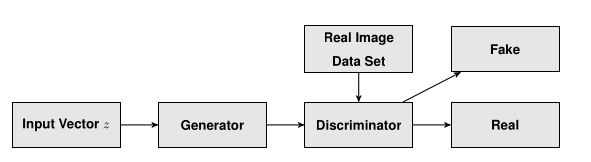
\includegraphics[scale=.45]{gan}
	\caption{GAN}
\end{figure}

$$
	\min_G\max_D V(D,G) = E_{x~p_{data}(x)}[log D(x)] + E_{z~p_z(z)}[log(1 - D(G(z)))].
$$

\end{frame}

\begin{frame}{Introduction}

% Requirements for steganography
	\begin{itemize}
		\item<1-> Imperceptibility 
		\item<2->  Robustness 
		\item<3->  payload capacity 
	\end{itemize}
\end{frame}

\begin{frame}{Literature Review}

\section{Literature Review}
% cover synthesis
Different approaches to steganography
\begin{itemize}
	\item cover modification 
	\item cover synthesis: Fridrich, K.-C. Wu \& Wang
\end{itemize}

\end{frame}

\begin{frame} {Literature Review}

% GANs in stego
Volkhonskiy, Shi, Dong,Tang,Hayes
\end{frame}

\begin{frame}{Literature Review}
	\subsection{SWE}
	% Ke
	Ke
\end{frame}

\begin{frame}{Literature Review}
	% Hu
	Hu
\end{frame}

\begin{frame}{Literature Review}
	% Zhang
	Zhang
\end{frame}

\begin{frame}{Problem Statement}
	\section{Problem Statement}
	% problem statement
	
	Observed problems: 
	\begin{itemize}
		\item Instability of Training
		\item Slow convergence
		\item Inadequately realistic image generation
	\end{itemize}

\pause
\textbf{\textquotedblleft This is mainly associated to the GAN technique used in the
	framework.\textquotedblright}
\end{frame}

\begin{frame}{Objectives}
	\section{Objectives}
	%general objectives
	Design and implement a powerful generative steganographic framework using a
most suitable GAN.
\end{frame}

\begin{frame}{Objectives}
	
	%specific objectives
	Specific objectives:
	\begin{itemize}
		\item Improve stability of Training and convergence speed.
		\item Generate more realistic image.
		\item Maintain state of the art security.
	\end{itemize}
	
\end{frame}

\begin{frame}{Methodology}
	\section{Methodology}
	% system architecture
	\begin{figure}
		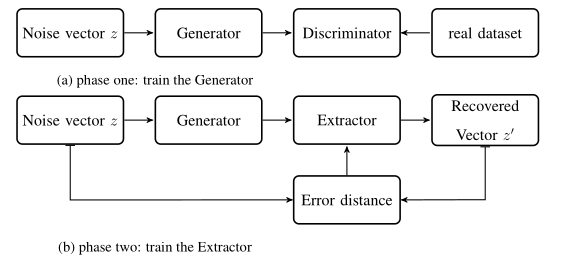
\includegraphics[scale=.45]{arch}
		\caption{System Architecture}
	\end{figure}
\end{frame}

\begin{frame}{Methodology}

	% choice of GAN
	Choice of GAN: 
	\begin{itemize}
		\item BEGAN
		\item RGAN
		\item WGAN-DIV
		\item WGAN-GP
	\end{itemize}
\end{frame}

\begin{frame}{Methodology}

 % choice of dataset
 Choice of dataset:
 \begin{itemize}
 	\item CelebA
 	\item LFW
 	\item Food101
 	\item MNIST
 \end{itemize}
\end{frame}

\begin{frame}{Methodology}
	
	% testing methods
	Choice of dataset:
	\begin{itemize}
		\item Visual instpection
		\item Inception score
		\item Visual Turing test
		\item MOS
	\end{itemize}
\end{frame}

\begin{frame}{Scope}
\section{Scope}
\begin{itemize}
	\item <1-> Robustness
	\item <2-> Passive Adversary
	\item <3-> Payload Capacity
	\item <4-> Imperceptibility
\end{itemize}
\end{frame}

\begin{frame}{Significance Of The Study}
\section{Significance Of The Study}
	The main problem in generative steganography 
	
	\begin{center}
		\textbf{Imperceptibility}
	\end{center}
\end{frame}


\begin{frame}{Work Plan}
\section{Work Plan}

\end{frame}

\begin{frame}{Budget}
\section{Budget}

\end{frame}

\begin{frame}
\begin{center}
\LARGE
THANK YOU
\end{center}
\end{frame}
\end{document}